\section{Auswertung}
\label{sec:Auswertung}

\subsection{Überprüfung der Stabilität}
\label{subsec:stabilitaet}
Die Messwerte für den realisierten Laser mit einem flachen und einem sphärischen
Spiegel befinden sich in Tabelle \ref{tab:plankonkav}. In Abbildung \ref{fig:plankonkav}
sind die gemessenen Stromstärken $I$ gegen die Resonatorlängen $L$ aufgetragen.
Zudem wird eine lineare Ausgleichrechung der Form
\begin{equation*}
  f(L)=a L+b
\end{equation*}
durchgeführt. Für die Parameter $a$ und $b$ ergeben sich die Werte
\begin{align*}
  a&= \SI{2.61(029)}{\micro\ampere\per\centi\per\metre}\,,\\
  b&= \SI{214(18)}{\micro\ampere}\,.
\end{align*}

\begin{figure}
  \centering
  \includegraphics{build/plankonkav.pdf}
  \caption{Darstellung der Messwerte sowie einer gefitteten Ausgleichsfunktion für den
  Resonator aus einem flachen und einem sphärischen Spiegel.}
  \label{fig:plankonkav}
\end{figure}

Die Messwerte für den Resonator aus zwei sphärischen Spiegeln befinden sich in
Tabelle \ref{tab:konkavkonkav}. In Abbildung \ref{fig:konkavkonkav} sind die gemessenen Stromstärken gegen die Resonatorlänge aufgetragen. Außerdem wird eine
Ausgleichsrechnung der Form
\begin{equation*}
  f(L)=a L^2 + b L + c
\end{equation*}
durchgeführt. Es ergeben sich die Parameter
\begin{align*}
  a&= \SI{0.097(017)}{\micro\ampere\per\centi\per\metre\squared}\,, \\
  b&= \SI{-21(4)}{\micro\ampere\per\centi\per\metre}\,, \\
  c&= \SI{1.15(020)e3}{\micro\ampere}\,.
\end{align*}

\begin{figure}
  \centering
  \includegraphics{build/konkavkonkav.pdf}
  \caption{Darstellung der Messwerte sowie einer gefitteten Ausgleichsfunktion für den
  Resonator aus zwei sphärischen Spiegeln.}
  \label{fig:konkavkonkav}
\end{figure}

\subsection{Vermessung der Moden}
\label{subsec:moden}

Die gemessenen Werte für die $TEM_{0,0}$ Mode befinden sich in den Tabellen \ref{tab:tem00a} und \ref{tab:tem00b}. In Abbildung \ref{fig:tem00} sind sie
grafisch dargestellt. Die Werte zeigen nicht den theoretisch zu erwartenden gaußförmigen
Verlauf. In Abbildung \ref{fig:bild} ist ein Bild dieser Mode eingefügt. Auch dort
ist im Zentrum eine geringere Intensität zu erkennen.

Trotz der Abweichungen wird eine gaußförmige Ausgleichsrechnung der Form
\begin{equation*}
  I_{0,0}(L)=I_{\text{max}} \exp\left(-2*\left(\frac{L-d}{\omega}\right)^2\right)
\end{equation*}
durchgeführt. Dabei ist $I_{\text{max}}$ der maximale Strom, $d$ eine Verschiebung in
x-Richtung und $\omega$ der Strahlradius.  Es ergeben sich die Parameter
\begin{align*}
  I_{\text{max}}&=\SI{597(29)}{\micro\ampere} \,,\\
  d&= \SI{-3.2(8)}{\milli\metre} \,, \\
  \omega&=\SI{27.8(17)}{\milli\metre} \,.
\end{align*}

\begin{figure}
  \centering
  \includegraphics{build/tem00.pdf}
  \caption{Darstellung der Messwerte sowie einer gefitteten Ausgleichsfunktion für die $TEM_{0,0}$ Mode.}
  \label{fig:tem00}
\end{figure}

\begin{figure}
  \centering
  \includegraphics[width=0.7\textwidth]{data/tem00.png}
  \caption{Bild der $TEM_{0,0}$ Mode. Deutlich zu erkennen ist eine schwächere Intensität im Zentrum.}
  \label{fig:bild}
\end{figure}


Die Messwerte für die $TEM_{0,1}$ Mode sind in den Tabellen \ref{tab:tem01a} und \ref{tab:tem01b} aufgeführt. In Abbildung \ref{fig:tem01} sind sie grafisch dargestellt. Es wird eine Ausgleichsrechnung
der Form
\begin{equation*}
  I_{0,1}=I_max\left(\frac{L-d}{\omega}\right) \exp\left(-2\left(\frac{L-d}{\omega}\right)^2\right)
\end{equation*}
durchgeführt.
Die Ausgleichsrechnung liefert die Parameter
\begin{align*}
  I_{\text{max}}&=\SI{1.27(05)e3}{\nano\ampere} \,,\\
  d&=\SI{0.38(28)}{\milli\metre} \,,\\
  w&=\SI{15.0(4)}{\milli\metre} \,.
\end{align*}

\begin{figure}
  \centering
  \includegraphics{build/tem01.pdf}
  \caption{Darstellung der Messwerte sowie einer gefitteten Ausgleichsfunktion für die $TEM_{0,1}$ Mode.}
  \label{fig:tem01}
\end{figure}

\subsection{Messung der Polarisierung}
\label{subsec:polarisierung}

In Tabelle \ref{tab:polarisation} befinden sich die Messwerte zur Intensität des
Laserstrahls in Abhängigkeit von dem Winkel des Polarisationsfilters. Diese Werte
sind in Abbildung \ref{fig:polarisation} graphisch dargestellt. Es wird eine Ausgleichsfunktion der Form
\begin{equation*}
  f(\phi)=I_{\text{max}} cos^2(\phi+\delta)
\end{equation*}
durchgeführt. Diese liefert die Parameter
\begin{align*}
  I_{\text{max}}&=\SI{56.02(118)}{\micro\ampere} \,, \\
  \delta&=\SI{919.32(105)} \,.
\end{align*}

\begin{figure}
  \centering
  \includegraphics{build/polarisation.pdf}
  \caption{Darstellung der Messwerte sowie einer gefitteten Ausgleichsfunktion für die Intensität in
  Abhängigkeit vom Winkel des Polarisationsfilters.}
  \label{fig:polarisation}
\end{figure}


\subsection{Bestimmung der Wellenlänge}
\label{subsec:wellenlaenge}
